\documentclass[submit,ses,noauthor]{ipsj} % SES スタイルを適用

\usepackage[dvipdfmx]{graphicx}
\usepackage{latexsym}
\usepackage{fancyhdr}

\def\Underline{\setbox0\hbox\bgroup\let\\\endUnderline}
\def\endUnderline{\vphantom{y}\egroup\smash{\underline{\box0}}\\}
\def\|{\verb|}



\begin{document}
\title{依存関係の向きを考慮したファイルの変更時間への影響分析}

\etitle{}

\affiliate{SU}{島根大学\\
Shimane University}


\author{上田 裕己}{Ueda Yuki}{SU}[s133014@matsu.shimane-u.ac.jp]

\begin{abstract}
大規模なソフトウェア開発では多くのファイルからソフトウェアが成り立っている.
そのため,あるファイルを変更した場合ほかのファイルにも影響を及ぼす.

既存研究では依存関係がソフトウェアの品質や開発者の経験に影響を与えることがわかっている.

本研究では,変更されたソースコードの依存関係の依存の向きに着目して,依存関係をもつファイルが次に変更されるまでの期間への影響を調査した.
 
実験結果から変更されているソースコードに依存関係の向きや変更を行った人物によって開発期間に大きく影響を与えることが分かった.
  

\end{abstract}

\maketitle

%はじめに
\section{はじめに} 
現在開発者の経験を図るために多くの研究で開発者がいままでに変更したファイルが利用されている.
Bird\cite{Bird}らは専門レベルをというあるファイルに対してどれだけ詳しいかによってソフトウェアの故障率が下がるという研究を行った.


しかし,対象ファイル群が依存する他のファイル群(以降,依存ファイル群)に対する専門レベルは考慮されていない.これは,依存ファイルと依存関係にあるファイルに対して十分な検査が行えず,不具合を見逃す恐れがある.

ファイルがもたらす影響の指針としては開発期間がある.


開発期間が分かればどのような依存関係のあるファイルに開発者が注目すればいいのかがわかることが予想される.


そのため,本論文では変更されたファイルに対して依存関係のあるファイルが変更されるまでの期間への影響を分析する.

そのために変更が行われたファイルに対してどのような関係を持っているのかプロジェクトの中で6つに分類を分けそれぞれへの影響を調査する.

これにより, 変更




本論文では\ref{関連研究}章で関連研究について書き\ref{調査方法}章で調査方法,\ref{実験結果}章で実験の結果,\ref{考察}章で実験結果についての考察,\ref{妥当性の検証}章では実験の妥当性についての検証,最後に\ref{まとめ}章でまとめを行う.


%関連研究
\section{関連研究}\label{関連研究}

Briandらは依存関係が変更までの時間に影響を与えることを調査した.

この研究では,変更されたファイルに対して依存しているファイルのみを調査している.

この問題点は変更されたファイルに対して依存されているファイルに対して調査が行われていない.
これにより,同じ機能を重複して実装したり, 機能を抽象化するさいの変化を終えていない可能性がある.

そこで,我々は依存されているファイルを同様に調査することによって依存関係の向きも考慮した.




\subsection{バージョン管理システム}
バージョン管理システムとはファイルの変更の履歴を保存するためのシステムである.
現在多くのソフトウェアではバージョンコントロール管理システムが利用されている.
GitHubなどの分散型のバージョン管理システムでは,多くの開発者が一つのソフトウェアを変更していても,変更の重複を防ぐことができる.


\subsection{doxygen}
コードの情報についてXML形式で出力するツール.
本研究ではvertプロジェクトで利用されているjavaで書かれたソースコードを解析するのに利用した.

                                                                                                                                                                                                                                                                                                                                                                                                                                                                                                                                                                                                                                                                                                                                                                                                                                                                                                                                                                                                                                                                                                                                                                                                                                                                                                                                                                                 
\section{調査方法}\label{調査方法}
以下の項目について調査を行う.
\begin{itemize}
\item RQ1:依存関係の種類によるコードファイルの変更時間
\item RQ2:変更する人物の傾向
\item RQ3:マージされたコミットの傾向
\end{itemize}

\subsection{調査対象のデータセット}
GitHub上のeclipseプロジェクトの中で最もstar数が多かったvert.vプロジェクトを調査,
vert.vプロジェクトは2013年から2016年まで変更され続け,合計2000以上のコミットが行われている.
eclipseプロジェクトには多くのオープンソースソフトウェアがあり,今後ほかのプロジェクトと比較するのに適していると考えた


\subsection{RQ1:依存関係の種類によるコードファイルの変更時間}
依存関係に種類を定義することによってどの種類がコードファイルの変更時間に影響を与えるのか調査を行った.
まずは,依存関係の
依存関係の距離にも着目した直接的に依存しているものと依存しているファイルに依存しているファイルというような間接的な依存関係にはdependee2といったように2をつけている.


また,本研究ではソースコードのうち以下のような記述を依存として扱う.
\begin{itemize}
\item 参照による代入や呼び出し(例:ClassA a = new ClassA())
\item 継承 (例: ClassA extends ClassB)
\end{itemize}


\subsubsection{依存関係の分類}
依存関係があるファイルにも依存関係の方向や間接的な依存関係をもつものを考慮するためにプロジェクト内のすべてのファイルを表\ref{tab:依存関係の分類}に示したような分類に分ける.
本論文ではこの分類を依存関係の分類と呼ぶことにする.図\ref{fig:dependency}に依存関係の分類についての図を用意した.

\begin{table}
\caption{依存関係の分類}
\begin{tabular}{|l|r|r|} \hline
分類名 & 概要 \\ \hline
root & 変更されたファイル \\ \hline
depender & rootが依存するファイル \\ \hline
dependee & rootが依存されるファイル \\ \hline
depender2 & dependerが依存するファイル \\ \hline
dependee2 & dependeeが依存されるファイル \\ \hline
other & 上記に当てはまらないファイル \\ \hline
\end{tabular}
\label{tab:依存関係の分類}
\end{table}

\begin{figure*}[t]
\centering
\includegraphics[width=2\columnwidth]{dependency.pdf}
\caption{依存関係の分類図}
\label{fig:dependency} 
\end{figure*}


\subsubsection{出力するデータセット}
csv形式で時系列とともに出力する.
出力するデータを表\ref{tab:初期データセット}に示した.


\begin{table}[htb]
\caption{出力するデータセット}
\begin{tabular}{|l|r|r|} \hline
属性名 & 概要 \\ \hline
filepass & ファイルの絶対パス \\ \hline
commitNo & HEADからのコミットの距離 \\ \hline
date & 変更が行われた日付 \\ \hline
author & 変更を行った開発者の名前 \\ \hline
kind & 依存関係の種類 \\ \hline
ismerge & マージされた後のコミットであるかどうか \\ \hline
\end{tabular}
\label{tab:初期データセット}
\end{table}

filepassとは出力するファイルのファウルパスである.
同一のcommitNoに対してその時点でのプロジェクトでのjavaファイルをすべて出力している.
このファイルパスは一意ではなく,同じfilepassとcommitNoでもkindが

commitNoとは

dateとは

authorとは

kindとは

ismergeとはコミットがmergeされたコミットかどうかを分類しているものであり,論理型の値を得る.

図{fig:gitimage} にコミットの分類を図示する.
このうちismergeがTrueとなるのは1と2のコミットである.

\begin{figure*}[t]
\centering
\includegraphics[width=2\columnwidth]{git_image.pdf}
\caption{gitによるコミットの分類分け}
\label{fig:gitimage} 
\end{figure*}




これらの情報をもとにさらにデータを追加する.
以下の表\ref{tab:加工後データセット}は上のデータをもとに算出するデータである.

\begin{table}[htb]
\caption{加工後データセット}
\begin{tabular}{|l|r|r|} \hline
属性名 & 概要 \\ \hline
SubDate & 依存関係が発生してから次に変更されるまでの日にち \\ \hline
SubCommitNo & 依存関係が発生してから次に変更されるまでのコミット数 \\ \hline
\end{tabular}
\label{tab:加工後データセット}
\end{table}

SubDateとは

SubCommitNoとは


以下の手順でデータ取得を行う.
\begin{enumerate}
\item プロジェクトの状態を一つ過去のものに戻す.
\item プロジェクトの情報をdoxygenで生成する
\item 生成されたXMLファイルから依存関係を求める.
\item 依存関係のあるファイルの情報をcsvファイルに出力する.
\item 過去の変更がなくなるまで1に戻る
\end{enumerate}

これにより得られたデータ量は141MGとなった.


%実験結果
\section{実験結果}\label{実験結果}
依存関係の分類別,またmergeされたかどうかによって依存関係を持つファイルが次に変更されるまでの日にち,コミット数を出力した.


%実験・RQ1
図\ref{fig:subNo},\ref{fig:subdate}はそれぞれ依存関係別にみた依存関係の検出から変更されるまでのコミット数や,日数を箱ひげ図で出力したものである.  

\begin{figure}
\centering
\includegraphics[width=\columnwidth]{CommitNo.pdf}
\caption{依存関係の分類ごとの次回変更までの変更回数}
\label{fig:subNo} 
\end{figure}

\begin{figure}
\centering
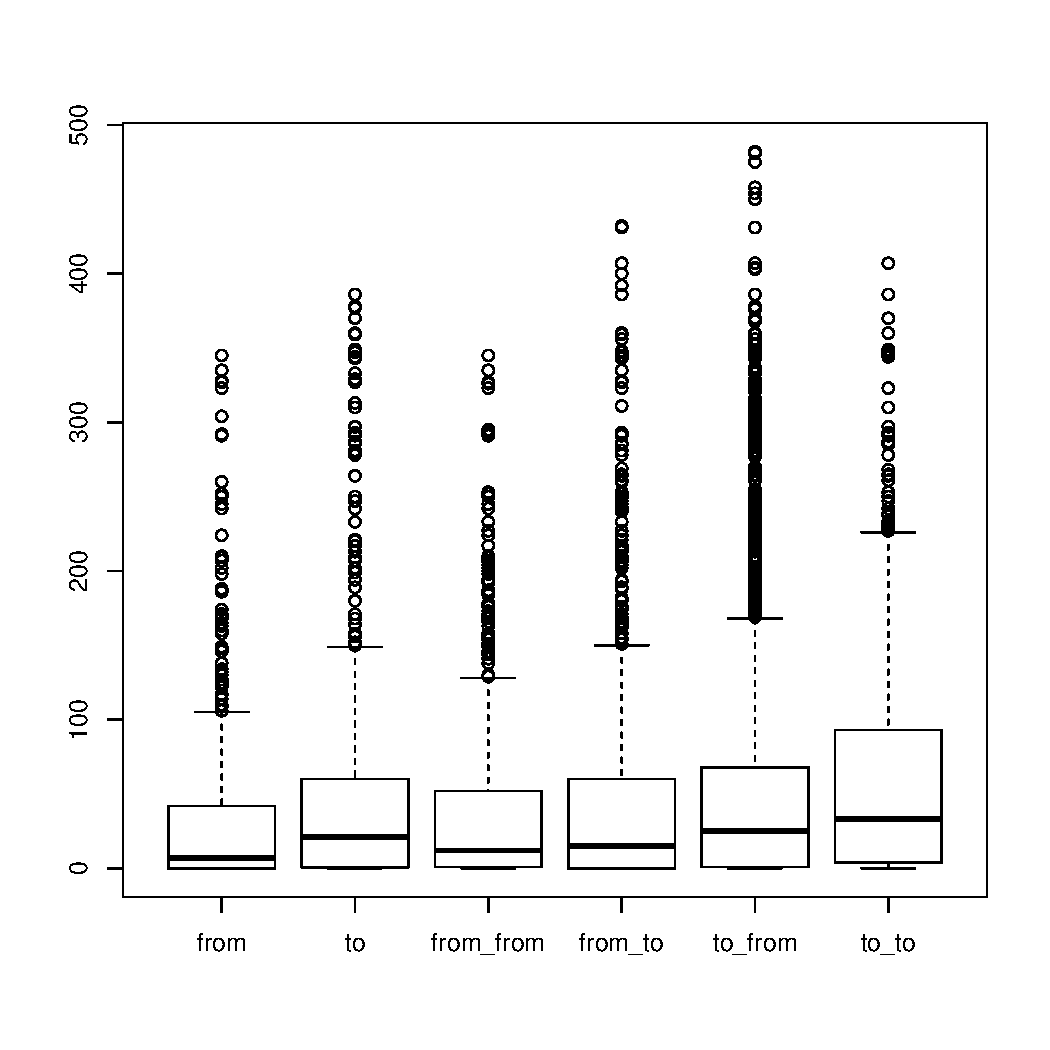
\includegraphics[width=\columnwidth]{date.pdf}
\caption{依存関係の分類ごとの次回変更までの変更日時}
\label{fig:subdate} 
\end{figure}


%実験・RQ2
\subsection{RQ2:変更する人物の傾向}
依存関係をもつファイルを同じ開発者が変更した場合の開発の期間への影響を調査した.
図の\ref{fig:author_true_subNo},\label{fig:author_true_subdate} はそれぞれ同じ開発者が変更した場合のSubCommitNo, Subdateを出力している.
また,図の\ref{fig:author_false_subNo},\label{fig:author_false_subdate} はそれぞれ異なる開発者が変更した場合のSubCommitNo, Subdateを出力している.


\begin{figure}
\centering
\includegraphics[width=\columnwidth]{author_CommitNo_TRUE.pdf}
\caption{同じ開発者の依存関係の分類ごとの次回変更までの変更回数}
\label{fig:author_true_subNo} 
\end{figure}

\begin{figure}
\centering
\includegraphics[width=\columnwidth]{author_CommitNo_FALSE.pdf}
\caption{異なる開発者の依存関係の分類ごとの次回変更までの変更回数}
\label{fig:author_false_subNo} 
\end{figure}

\begin{figure}
\centering
\includegraphics[width=\columnwidth]{author_date_TRUE.pdf}
\caption{同じ開発者の依存関係の分類ごとの次回変更までの日数}
\label{fig:author_true_subdate} 
\end{figure}

\begin{figure}
\centering
\includegraphics[width=\columnwidth]{author_date_FALSE.pdf}
\caption{異なる開発者の依存関係の分類ごとの次回変更までの日数}
\label{fig:author_false_subdate} 
\end{figure}


%実験・RQ3
\subsection{RQ3:マージされたコミットの傾向}
mergeされた変更の開発の期間への影響を調査した.
図の\ref{fig:merge_true_subNo},\label{fig:merge_true_subdate} はそれぞれmergeされた変更のSubCommitNo, Subdateを出力している.
また,図の\ref{fig:merge_false_subNo},\label{fig:merge_false_subdate} はそれぞれmergeされていない変更のSubCommitNo, Subdateを出力している.


\begin{figure}
\centering
\includegraphics[width=\columnwidth]{merge_CommitNo_TRUE.pdf}
\caption{mergeされたコミットの依存関係の分類ごとの次回変更までの変更回数}
\label{fig:merge_true_subNo} 
\end{figure}

\begin{figure}
\centering
\includegraphics[width=\columnwidth]{merge_CommitNo_FALSE.pdf}
\caption{mergeされていないコミットの依存関係の分類ごとの次回変更までの変更回数}
\label{fig:merge_false_subNo} 
\end{figure}



\begin{figure}
\centering
\includegraphics[width=\columnwidth]{merge_date_TRUE.pdf}
\caption{}
\label{fig:merge_true_subNo} 
\end{figure}

\begin{figure}
\centering
\includegraphics[width=\columnwidth]{merge_date_FALSE.pdf}
\caption{}
\label{fig:merge_false_subNo} 
\end{figure}


%考察
\section{考察}\label{考察}

\subsection{RQ1:依存関係の種類によるコードファイルの変更時間}
図\ref{fig:subdate}と図\ref{fig:sub}について考察する.

最も開発期間が長いものがotherであることから依存関係があるものは依存関係の向きや長さを問わず早く変更される傾向にあると考えられる.


dependeeやdependee2からわかるように変更されたファイルに依存しているファイルが早く変更される傾向にあることが分かった.
すべてのファイルの変更されるまでの日付の中央値は25日なのに対してdependeeは約5日で変更される.
このことから依存関係の距離よりも依存関係の向きが開発機関に影響を与えることが分かった.
.

dpendeeが早い段階で影響を受けていることが分かった.


以上から,影響があるのは順に依存関係の向き,依存関係の距離が関係していることがわかる.



\subsection{RQ2変更する人物の傾向}
図\ref{fig:author_true_subNo} から\ref{fig:author_false_subdate} について考察する

同じ人物が変更した場合と比較し,違う人物が変更したファイルは全体的に中央値が高い結果になっている.
depender2とotherを比較した場合,違い人物が変更した場合には大きな差がないのに対して,同じ人物が変更した場合は20日近く差があることが分かった.

同じ人物が変更した場合に中央値が下がることに関して考えられることは,同じ開発者が変更したコミットの大部分は同時に変更をしたものである.
多くの開発者が不具合がでないように他の依存関係のあるファイルを変更するので妥当な結果といえる.

別の開発者が変更をした場合にはdepender2とotherに対して大きく差がでる.

これは同じパッケージに入っているために影響がでることが考えられる.


\subsection{RQ3:マージされたコミットの傾向}
図\ref{fig:merge_true_subNo} から\ref{fig:merge_false_subNo} について考察する

マージされたコミットほど変更されるタイミングが遅くなる.
また,マージされていないコミットではdepender2とotherとの差がないことがわかった.



mergeされたコミットの場合mergeされていないコミットと比較して次に変更される時期が遅くなる傾向がある.
以下はその理由を考察た.
\begin{enumerate}
\item レビューを通してから変更を適用するために信頼性が高く,変更の必要がなくなる
\item mergeされ終わり, 作業が減る
\item 変更を行ったのがコアコミッターではないため不具合があったとしても修正に時間がかかる
\end{enumerate}

特にmergeされたコミットではdepender2はotherと中央値が近い数値を出している.
以下に理由について考察した.

\begin{enumerate}
\item 外部からの変更ではあまり抽象的になりがちなファイルを変更しづらい
\item 絶対数が少ないため, 変更されにくい
\end{enumerate}

\section{妥当性の検証}\label{妥当性の検証}
次に,妥当性について検証を行う.

\begin{itemize}
\item 今回の実験で用いたプロジェクトはオープンソースである,eclipseプロジェクトである.
ほかのオープンソースプロジェクトや商業ソフトウェアで,同様結果が得られるとは限らない.

\item 依存関係についての調査では継承や参照もすべて同じ依存関係であるとした.
これらを同じように扱うことで別のデータに偏りが発生した可能性がある.
\end{itemize}


\section{まとめ} \label{まとめ}
本研究では,ファイルの依存関係が位階の変更にどのような時間の影響を受けるか調査した.
その結果,依存関係の向きや距離,開発者によって開発期間に変化が現れることが分かった.

また,mergeされていないコミットほど早いく変更されやすいことからレビューを行っていない変更の場合は特に依存関係に注意をする必要がある.
今回は一つのプロジェクトのみを調査した.ほかのプロジェクトでも同じような傾向がみられるか調査する必要がある.



\begin{thebibliography}{10}
\bibitem{Bird}
Bird, Christian, et al. "Don't touch my code!: examining the effects of ownership on software quality." Proceedings of the 19th ACM SIGSOFT symposium and the 13th European conference on Foundations of software engineering. ACM, 2011.
\bibitem{Balachandram}
V. Balachandran: Reducing Human Effort and Improving Quality in Peer Code Reviews using Automatic Static Analysis and Reviewer Recommendation, ICSE'13, pp. 931-940, 2013.
\bibitem{Thongtanunam}
Patanamon Thongtanunam, Chakkrit Tantithamthavorn, Raula Gaikovina Kula, Norihiro Yoshida, Hajimu Iida, Ken-ichi Matsumoto: Who Should Review My Code? A File Location-Based Code-Reviewer Recommendation Approach for Modern Code Review, 22nd IEEE International Conference on Software Analysis, Evolution, and Reengineering, 2015.
\bibitem{Thongtanunam2}
Patanamon Thongtanunam and Shane McIntosh and Ahmed E. Hassan and Hajimu Iida: Revisiting Code Ownership and Its Relationship with Software Quality in the Scope of Modern Code Review, Proc. of the International Conference on Software Engineering (ICSE), 2016
 \end{thebibliography}

\end{document}
